\chapter{The Early Universe}
\hspace{0.5cm} The shortcoming  of FRW cosmology is that it is unable to explain why the universe we observe is homogeneous and isotropic on larger scales  without a finely tuned set of initial conditions, and how the initial seed perturbations for structure formation were generated.

In this chapter, we delve into two of the primary problems of the Hot Big Bang model: the horizon problem and the flatness problem. We explore how inflation, an early period of accelerated expansion, can drive the primordial Universe towards homogeneity and isotropy, even if it begins in a more generic initial state, and also how quantum fluctuations that arise during the inflationary period can give rise to the formation of primordial black holes.

\section{The Horizon Problem}
\hspace{0.5cm}Previously we introduced Hubble radii ($r_H = (aH)^{-1}$) Eq.\ref{eq:1.33} and comoving particle horizon $\tau$ \ref{eq:1.28} as an integral of the comoving Hubble radii. We could observe that for a universe dominated by the fluid equation of state, $w > -1/3 $ the Hubble radius  and the comoving particle horizon grow monotonically with time which implies that the comoving scales entering the horizon today have been far outside the horizon at CMB decoupling. But we find the CMB to be extremely homogeneous. In other words, at the time of the last scattering, the universe was expected to be homogeneous only on small scales since wider scales would not have been causally connected. However, the observation of the nearly homogeneous CMB suggests that the universe was extremely uniform even on larger scales that should have been independent of each other which was surprising.\\
\hspace{0.5cm}To overcome the horizon problem, it's important to consider the causal contact between particles. If a region, denoted by $\lambda$, has a typical size (constant in comoving scales) that is smaller than $(a_{I}H_{I})^{-1}$, then the particles within that region were in causal contact. However, if $\lambda$ becomes larger than $(a_{I}H_{I})^{-1}$ after a sufficient period of inflation, then these particles can no longer communicate. Therefore, before crossing the Hubble radius and becoming causally disconnected, these particles had the opportunity to communicate with each other and reach similar conditions. This implies that everything within the Hubble sphere at the beginning of inflation, which is $(a_{I}H_{I})^{-1}$, was in causal contact.\\
\hspace{0.5cm} We can hence observe that  the horizon problem can be resolved if the comoving Hubble radius at the beginning of inflation, $(a_I H_I)^{-1}$, exceeds the radius of the observable universe, $(a_0 H_0)^{-1}$. In this scenario, the entire observable universe would have been contained within the comoving Hubble radius at the onset of inflation.\\
The duration of the inflation to solve the horizon problem is given by the means of e-folds which is defined as,
\begin{align}
    \mathcal{N} = ln \left( \frac{a_E}{a_I} \right)
\end{align} \label{2.1}
from the requirement  $(a_I H_I)^{-1} > (a_0 H_0)^{-1}$ we get $\mathcal{N} \approx 60 $
\begin{figure}[h]
    \centering
    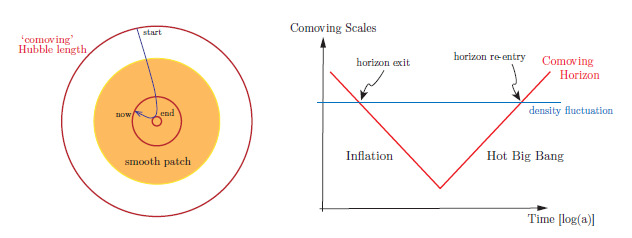
\includegraphics[width=0.7\textwidth]{horizon.png}
    \caption{\emph{Left}: Development of the inflationary universe's $(aH)^{-1}$ comoving Hubble radius. Inflation causes the co-moving Hubble sphere to contract and then expand. Hence, inflation serves as a tool to "zoom in" on a smooth sub-horizon patch. \emph{Right}: Solution of the horizon problem. All scales that are relevant to cosmological observations today were larger than the Hubble radius until $a \sim 10^{-5}$. These scales were, however, smaller than the Hubble radius at sufficiently early eras and were consequently causally related. Similarly, the scales of cosmological interest came back within the Hubble radius in relatively recent times.\cite{baumann2012tasi}}
    \label{fig:2.1} 
\end{figure}

\section{The Flatness Problem}
We saw in  section \ref{section 1.4} that the current measurements of the density parameters are compatible with a flat universe $\Omega_{total} \simeq 1 $.But the question arises how does $\Omega $ evolve with time?
We can write the Friedmann equation \ref{eq:1.43} as 
\begin{align}
    \Omega(t)-1 = \frac{k}{H(t)^{2} a(t)^{2}} \propto  \frac{k}{a^{2-3(1+w)}} = ka^{3w+1} \label{2.2}
\end{align}
We observe that for both radiation ($w = 1/3$) and matter ($w = 0$), we see that if $\Omega - 1 \neq 0$ at a certain early time then it will grow as $a^2$ or 
$a^4$ respectively and then the geometry of the present Universe is expected to be curved. So the near-flatness, we observe today requires the value of $\Omega(t)$ to be one. \\
By manipulating the Friedmann equation \ref{eq:1.43} we find

\begin{align}
  \Omega ^{-1} (z) -1
  = (\Omega_0 ^{-1} -1)\qty(\frac{T_0 }{T(z)})^{2} \,.
\end{align}

Let us extend this to the Planck epoch because the density at a time $t_P \approx 10^{-43}s$ must have been very close to the critical density. The temperature at that time was $T_P = \num{e32} K $. $T_{0}$ is the temperature today.


If we compute \(T _{\text{Pl}} / T_0 \) we get approximately \num{e32}.

This means that 
\begin{align}
    \Omega^{-1}(z_{\text{Pl}}) - 1 \approx (\Omega_0^{-1} - 1) \num{e-64}\,.
\end{align}
.As a result, the Universe should have needed to be extraordinarily finely tuned in order to imitate the flatness we observe today.

Using the Hubble radius, we can write to examine how the inflationary phase responds to this issue.
\begin{align}
    \Omega(t)-1 = \frac{k}{H(t)^{2} a(t)^{2}} = kr_{H}^2
\end{align}
In standard cosmology, the comoving Hubble radius grows with time,
therefore one expects the quantity $|\Omega(t)-1|$ to grow with time and the geometry of the present Universe to be curved. But,
if the universe undergoes a phase where the Hubble radius shrinks, this would bring $\Omega(t)$ closer to 1. It can be shown that the universe must expand by 60 e-foldings to achieve the flatness we observe today, as in the case of the horizon problem.



\section{Dynamics of Inflation}

\hspace{0.5cm}In the previous section, we saw that for inflation to take place we need  a phase of accelerated expansion ($\ddot{a} > 0$) where the Hubble radius($r_{H}$) shrinks.\\
We can see from the Friedmann Eq. \ref{eq:1.21a} that for an accelerated expansion
\begin{align}
    \ddot{a} = -\frac{4 \pi G}{3}(\rho+3P) > 0 \Rightarrow P < \frac{-\rho}{3}\,\label{2.6}
\end{align}
which we previously encountered in the  de-Sitter model where we found $a(t) \propto exp(\sqrt{\frac{\Lambda}{3}}t)$ and the expansion is driven by cosmological constant $\Lambda$, so we can have a calculated guess that the inflation can't be driven by matter or radiation. In the current  interpretation, $\Lambda$ is linked to the quantum fluctuations of the vacuum. The  vacuum expectation value of the stress-energy tensor gives the energy generated by these fluctuations.Using Eq. \ref{eq:1.19} and Eq. \ref{1.32} we can write
\\
\begin{align}
    \langle T_{\mu\nu} \rangle = -\langle P_{\Lambda} \rangle g_{\mu\nu} = \frac{\Lambda}{8\pi G} g_{\mu\nu} \label{2.7}
\end{align}
As a result, in this instance, the stress-energy tensor's vacuum expectation value functions as the cosmological constant that promotes the expansion. This provides an indication of what to anticipate from a theory describing the inflationary mechanism.

\subsection{Scalar(Inflaton) Field }





\hspace{0.5cm}To satisfy Eq. \ref{2.6} let us introduce a minimally coupled(i.e not coupled with gravity or any other field ) scalar field \(\varphi\)  with a suitable potential $V(\varphi)$ which is a self-interaction of the field. We can write its Lagrangian as 
\begin{align}
    \mathscr{L}_{\varphi} = -\frac{1}{2} g^{\mu\nu} \partial_{\mu}\varphi\partial_{\nu}\varphi - V(\varphi)\, \label{2.8}
\end{align}
The action is in the form of 

\begin{align}
    S = S_{EH} + S_\varphi + S _{\text{matter}}\,\label{2.9}
\end{align}

where \(S_{EH}\) is the Einstein-Hilbert action for the metric, \(S_\varphi \) is the action for the field \(\varphi \), while ``matter'' encompasses all the other fields but we can ignore it thanks to the \emph{no-hair cosmic theorem}.

\begin{align}
    S = \frac{1}{16 \pi G} \int \dd[4]{x} \sqrt{-g} R + \int \dd[4]{x} \sqrt{g} \mathscr{L}\varphi [\varphi , g{\mu \nu }],. \label{2.10}
\end{align}

We are using the invariant volume element \(\dd[4]{x} \sqrt{-g}\)
representing the physical 4-volume regardless of the coordinates.
Now, we can find the equation of motion for the inflaton field by  the Klein-Gordon equation by varying the action with respect to $\varphi$.
\begin{align}
    \square \varphi = \pdv{V}{\varphi }\,. \label{2.11}
\end{align}
where $\square$ is the covariant D'Alembert operator.
\begin{align}
    \square \varphi = \frac{1}{\sqrt{-g}} \qty(g^{\mu \nu } \sqrt{g} \varphi_{, \mu })_{, \nu }\,.\label{2.12}
\end{align}
and in a flat FRW metric Eq. \ref{eq:1.1} $\sqrt{-g} = a^3$ the evolution of $\varphi$ becomes
\begin{align}
    \square \varphi = \frac{1}{a^3} \partial_0 (g^{00} a^3\partial_0\varphi) + \frac{1}{a^3} \partial_i (g^{ii} a^3\partial_i\varphi) 
    &= \partial _{\varphi} V  \\ - \ddot{\varphi} - \dot{\varphi} 3\frac{\dot{a}}{a} + \frac{\nabla^2}{a^2} \varphi  
    &= \partial _{\varphi} V  \\ \ddot{\varphi} + 3 H \dot{\varphi} - \frac{\nabla^2 \varphi }{a^2} &= - \partial _{\varphi} V\,. \label{2.15}
\end{align}
where $3H\ddot{\varphi}$ appears as a friction term that is represented as a scalar field rolling down its potential suffering friction due to the expansion of the universe. If we consider the homogeneous background field, it will be constant in space, so  the above equation evolves as\\
\begin{align}
     \ddot{\varphi} + 3 H \dot{\varphi}  &= - \partial _{\varphi} V\,. \label{2.16}
\end{align}
The stress-energy tensor associated with the scalar field can be defined by 

\begin{align}
    T_{\mu \nu }^{(\varphi )} = - \frac{2}{\sqrt{-g}} \fdv{S_{\varphi }}{g^{\mu \nu }} =- 2 \frac{\partial\mathscr{L}_\varphi }{\partial g^{\mu \nu }} + \frac{2}{\sqrt{-g}} \mathscr{L}_\varphi \pdv{\sqrt{-g}}{g^{\mu \nu }} = - 2 \pdv{\mathscr{L}_\varphi }{g^{\mu \nu }} + \mathscr{L}_\varphi g_{\mu \nu }\\ = \partial_{\mu } \varphi \partial_{\nu } \varphi + g_{\mu \nu } \qty[- \frac{1}{2} g^{\alpha \beta } \partial_{\alpha } \varphi \partial_{\beta} \varphi - V(\varphi )] \,. \label{2.18}
\end{align}
If we compare it with Eq. \ref{eq:1.19} we find that $\varphi(t)$ behaves like a perfect fluid with
\begin{align}
    P &= -\frac{1}{2} g^{\alpha \beta }\partial_{\alpha } \varphi \partial_{\beta} \varphi - V(\varphi ) \label{2.19} \\
    \rho &= - \frac{1}{2} g^{\alpha \beta }\partial_{\alpha } \varphi \partial_{\beta} \varphi  + V(\varphi )  \label{2.20} \\
    u_\mu &= \frac{\partial_{\mu}\varphi}{\abs{\partial \varphi }}  \\
    \abs{\partial \varphi} &= \sqrt{- g^{\alpha \beta }\partial_{\alpha } \varphi \partial_{\beta} \varphi}
    \,.
\end{align}
\hspace{0.5cm}We start by considering $\varphi(t,x)$ and split it as
\begin{align}
    \varphi (\mathbf{x}, t) = \varphi(t) + \delta \varphi (\mathbf{x}, t) \, \label{2.23}
\end{align}
where $\varphi(t)$ is the classical field that is the expectation value of the inflaton field(\(\langle \varphi(t,x) \rangle = \varphi(t)\)) and $\delta \varphi(\mathbf{x}, t)\ $ represents the quantum fluctuations around $\varphi(t)$.
Now , 
\begin{align}
    \left|\frac{\delta \varphi(\mathbf{x}, t)}{\varphi(t)} \right| \ll 1 \label{2.24}
\end{align}
as quantum fluctuation is negligible in comparison to the classical value. These fluctuations are what generated the density fluctuation which creates anisotropies in the CMB photons. Let us drop the $"t"$ and indicate the value of the classic inflaton field by $\varphi$. On explicitly computing the energy-momentum tensor of the classical background $\varphi$ we find,
\begin{align}
    T^{0}_{0} &= - \qty( \frac{1}{2} \dot{\varphi}(t)^2 + V(\varphi )) = - \rho_\varphi\label{2.25}\\
    T^{i}_{j} &= \qty( \frac{1}{2} \dot{\varphi}^2 (t) - V(\varphi)) \delta^{i}_{j} = P_\varphi \delta^{i}_{j}\,. \label{2.26}
\end{align}
This is the perfect fluid energy-momentum tensor. Therefore, if 
\begin{align}
    V(\varphi) \gg \dot{\varphi}^2 ,\ \label{2.27}
\end{align}
we get $P_{\varphi} \simeq -\rho_{\varphi} \implies w_{\varphi} \simeq -1 $ i.e the quasi-de Sitter expansion.\\
So, we see that if the potential energy is greater than the kinetic energy  this scalar field gives inflation. For better intuition let us simplify the system and assume the vacuum expectation value of the inflaton to be constant i.e \(\langle \varphi(t,x) \rangle = \Bar{\varphi}\) then the stress-energy tensor becomes
\begin{align}
    \langle T_{\mu\nu} \rangle  = -g_{\mu\nu} V(\varphi) ,\ \label{2.28}
\end{align}
Comparing it to Eq. \ref{2.7} we see that the potential of the inflaton field $V(\varphi)$  represents the vacuum energy associated with $\varphi$ which drives the acceleration.\\

\subsection{Slow Roll Conditions}
\begin{figure}[h]
    \centering
    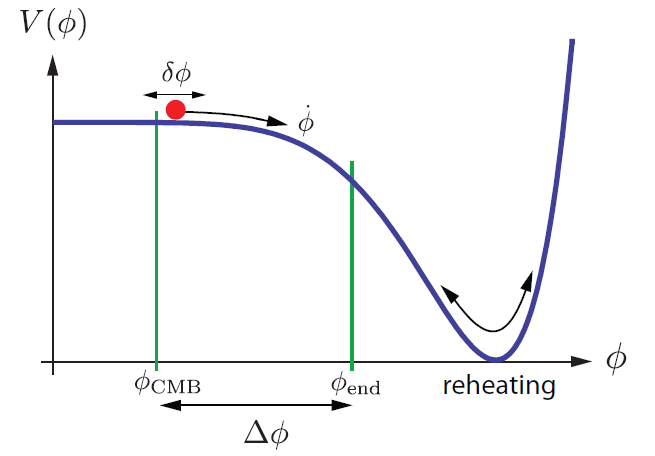
\includegraphics[width=0.7\textwidth]{inflaton.png}
    \caption{A possible shape of the potential for Slow-Roll Inflation \cite{baumann2012tasi}}
    \label{fig:2.2} 
\end{figure}
\hspace{0.5cm} Let us try to understand under what conditions the scalar field may initiate inflation. The equation of motion for the homogeneous scalar field is given in Eq. \ref{2.16}. To satisfy the condition given in Eq. \ref{2.27} the scalar field should slowly roll down its potential. The easiest way to satisfy the slow roll condition is to require that there exist regions of field-configuration space where the potential is sufficiently flat. Considering the potential to be flat the acceleration of the field should be negligible i.e
\begin{align}
    \ddot{\varphi} \ll 3H\dot{\varphi} \label{2.29}
\end{align}
We can also say as at a sufficiently late time the scalar field is driven by friction term. Therefore,
\begin{align}
    3H\dot{\varphi} \approx -\partial_{\varphi} V \label{2.30}
\end{align}
We expect that $V$ and all of its derivatives change very slowly with $\varphi$.
This means that in this equation we have \(\partial_{\varphi} V \approx const\), as well as \(H \approx const\): this is the same equation that is obeyed by a particle under a constant force and friction: it will then reach the asymptotic ``{terminal velocity}'' and move with a constant \(\dot{\varphi}_0 \).\\ 

So, the slow-roll condition is,
\begin{align}
     \ddot{\varphi} \ll (3H\dot{\varphi}),(-\partial_{\varphi} V )\label{2.31}
\end{align}\\
Let us now combine it with the Friedmann equation  \ref{eq:1.43},
\begin{align}
    H^2 = \frac{8 \pi G}{3} \qty(\rho _\varphi + \rho _m + \rho _r) - \frac{k}{a^2}\,.
\end{align}

The matter and radiation densities scale like \(a^{-3}\) for \(\rho _m\), \(a^{-4}\) for \(\rho _r\); in this early phase the scalar field dominates the dynamics, so the equation will simplify to 

\begin{align} \label{2.33}
    H^2 \approx \frac{8 \pi G}{3} V(\varphi)\,.
\end{align}
so, for a slow roll case, the Hubble parameter is nearly a constant and the scale factor is given by $a(t) \propto exp(Ht)$.\\
\hspace{0.5cm} We saw the slow roll conditions which are necessary for successful inflation. Next, we will parameterize it.

\
\hspace{0.5cm} These are the parameters we need to quantify in order to determine how closely the potential matches our expectations. It is given by $\epsilon$ and $\eta$. Let us start with the first parameter.\\
We define $\epsilon$ as,
\begin{align}
    \epsilon = -\frac{\dot{H}}{H^2}. \label{2.34}
\end{align}
As we saw previously for inflation to take place the Hubble radius shrinks. So let us write this in terms of the $\epsilon$ parameter.
\begin{align}
    \dv{(aH)^{-1}}{t} = \frac{-\dot{a}H + a\dot{H}}{(aH)^2} = -\frac{1}{a}\left( 1- \left( \frac{-\dot{H}}{H^2}\right)\right) = -\frac{1}{a}(1 - \epsilon) \label{2.35}
\end{align}
so we see that if $\dot{r_H} < 0$ implies that $\epsilon \ll 1 $.\\
\hspace{0.5cm} Using Eq. \ref{2.30} and Eq. \ref{2.33} we can write $\epsilon$ as,
\begin{align}
    \epsilon = - \frac{\dot{H}}{H^2} = + 4 \pi G \frac{\dot{\varphi}^2}{H^2} \approx \frac{3}{2} \frac{\dot{\varphi}^2}{V} = \frac{1}{16 \pi G} \qty(\frac{\partial_{\varphi} V}{V})^2\,,\label{2.36}
\end{align}
so the condition $\epsilon \ll 1 $ can also be written as 
\begin{align}
    \frac{(\partial_{\varphi} V)^2}{16 \pi G V^2} &\ll 1  \\ 
    \frac{(\partial_{\varphi} V)^2}{V} &\ll 16 \pi G V = \frac{2}{3} H^2 \\ 
    \frac{1}{V} \qty(\pdv{V}{\varphi })^2 &\ll H^2\,.\label{2.39}
\end{align}
on using Eq. \ref{2.34} we can see that it is exactly the slow roll condition in Eq. \ref{2.27}, So, we see that $\epsilon$ gives a bound on the first derivative of the potential and corresponds to the conditions of the potential being flat and the kinetic energy being small compared to the potential.\\
The second derivative of the potential is controlled by the parameter $\eta$ which is defined as,
 \begin{align}
     \eta = - \frac{\ddot{\varphi}}{H \dot{\varphi}}\,, \label{2.40}
 \end{align}
 and we can also define 

\begin{align}
    \eta = \frac{1}{3} \frac{\partial^{2} _{\varphi} V}{H^2} = \frac{1}{8 \pi G} \frac{\partial^{2} _{\varphi} V}{V} \,. \label{2.41}
\end{align}

We can see that \(\eta \ll 1 \) is equivalent to
\begin{align}
    \pdv[2]{V}{\varphi} \ll H^2 \label{2.42}
\end{align}

We can show that these three parameters are related  \(\delta = \eta - \epsilon \).\\
We start from Eq. \ref{2.30} and differentiate it with respect to the time we get 

\begin{align}
    \ddot{\varphi} &\approx - \dv{}{t} \qty( \frac{\partial_{\varphi} V}{3H})  \\ &= - \frac{1}{3H} \partial^{2} _{\varphi} V \dot{\varphi} - \frac{\partial_{\varphi} V}{3} \underbracket{\qty(- \frac{\dot{H}}{H^2})}_{\epsilon }  \\ &= - \dot{\varphi} H \frac{\partial^{2} _{\varphi} V}{3H^2} - \frac{\partial_{\varphi} V}{3} \epsilon  \\ &= - \dot{\varphi} H \eta - \frac{\partial_{\varphi} V}{3} \epsilon  \\ {-\frac{\ddot{\varphi}}{H \ddot{\varphi}}} &= \eta - \epsilon  \\
    \delta &= \eta - \epsilon,.\label{2.48}
\end{align}
which is the desired result.
We see that $\delta \ll 1 $ corresponds to the condition $\ddot{\varphi} \ll -\partial_{\varphi} V$, which is required in order to neglect the acceleration term in the Klein-Gordon equation. So, the condition  $\delta \ll 1 $ ensures that we move towards an attractor solution in the friction-dominated regime i.e, it will then reach the asymptotic “terminal velocity” and move with a constant $\dot{\varphi}$. Also, for inflation to solve the horizon and the flatness problem  we need a phase of accelerating expansion that lasts sufficiently long. For this to happen, we need $\epsilon \sim const$, since $\epsilon \sim \dot{\varphi}$ while $\delta \sim \ddot{\varphi}$, so requiring $\delta \ll 1$ also ensures this.
.\\
\hspace{0.5cm}In summary, the slow-roll approximation described in Eq. \ref{2.27} and Eq. \ref{2.31} implies the inflationary potential's flatness under conditions Eq. \ref{2.36} and Eq. \ref{2.41}.\\



\section{Inflation-Induced Cosmological Perturbations} \label{section 2.4}
 Inflationary cosmology relies on understanding the evolution of quantum fluctuations of the inflaton field $\delta \varphi(\mathbf{x},t)$, which give rise to primordial energy density perturbations that persist after inflation and form the basis of the large-scale structures observed in the Universe. These fluctuations arise on extremely small scales within the comoving Hubble radius during inflation, but the rapid expansion of space during this epoch stretches them out to cosmological scales. As the Hubble radius begins to increase faster than the scale factor after inflation ends, these fluctuations eventually re-enter the Hubble radius during the radiation or matter-dominated eras. The fluctuations that re-enter around 60 e-foldings before reheating have physical wavelengths that can be observed through various methods, such as the analysis of CMB anisotropies. The resulting inflationary spectrum provides a unique and distinct signature of inflation that can help us understand the origins of structure in the Universe. \\

 \begin{figure}[h]
    \centering
    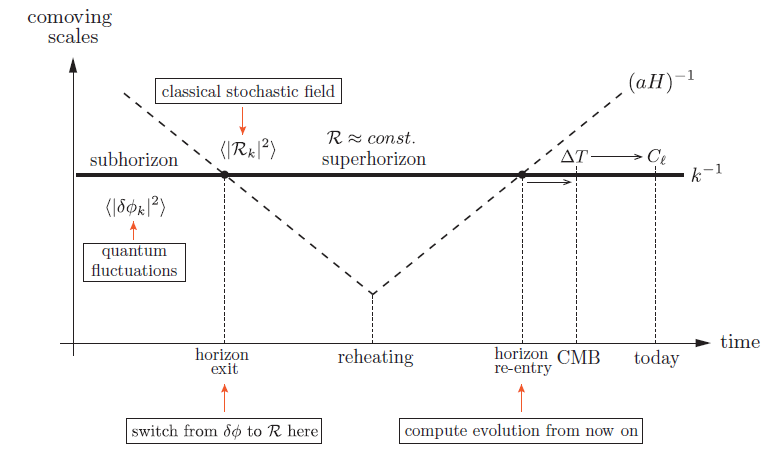
\includegraphics[width=0.7\textwidth]{comving vs conformal time.png}
    \caption{Creation and evolution of perturbations in the inflationary universe. On subhorizon scales, quantum mechanics produces fluctuations. During inflation, comoving scales, $k^{-1}$, stay constant in the comoving Hubble radius, but  $(aH)^-{1}$ diminishes and the perturbations leave the horizon, where they remain frozen until horizon re-entry at later times. The fluctuations change into anisotropies in the CMB and disturbances in the LSS after horizon re-entry. Taken from \cite{baumann2012tasi}}
    \label{fig:2.3} 
\end{figure}

\subsection{Dynamics of Quantum Fluctuations: Qualitative Analysis}

 \hspace{0.5cm} Let us now describe qualitatively how the quantum fluctuations of a generic scalar field evolve during an inflationary stage. We saw the dynamics of the scalar field obey the Klein-Gordon Eq. \ref{2.15} which we Taylor expand upto linear order around the background value for both $\varphi$ Eq. \ref{2.23} and for the potential \(V(\varphi ) \approx V_0 + \delta \varphi \eval{(\pdv{V}{\varphi })}_{\varphi_0 }\). Assuming the perturbation is indeed small we can write the Klein-Gordon equation for the fluctuation as

\begin{align} 
    \ddot{ \delta \varphi} + 3 H \dot{\delta \varphi} - \frac{\nabla^2}{a^2} \delta \varphi = - \pdv[2]{V(\varphi )}{\varphi } \delta \varphi \,. \label{2.49}
\end{align}
Let us move to the Fourier space which is more convenient for the problem. We can write,
\begin{align}
    \delta \varphi (\mathbf{x}, t) = \frac{1}{(2\pi )^{3}} \int \dd[3]{k} 
    e^{i \mathbf{k} \cdot \mathbf{x}} \delta \varphi _{\mathbf{k}}(t)
    \,.\label{2.50}
\end{align}
Since the field is real, \(\delta \varphi _{\mathbf{k}} = \delta \varphi _{- \mathbf{k}}^{*}\).\\
Now we will write the Klein-Gordon equation  for the quantum fluctuation in Fourier space.

\begin{align}
    \ddot{ \delta \varphi} _{\mathbf{k}} + 3 H \dot{ \delta \varphi}_{\mathbf{k}} + \frac{k^2}{a^2} \delta \varphi _{\mathbf{k}} = - \partial_{\varphi}^2(V) \delta \varphi _{\mathbf{k}}\,.\label{2.51}
\end{align}

If we consider a massless scalar field $\partial_{\varphi}^2(V) \approx 0$ which corresponds to the requirement of the parameter $\eta \ll 1$ which we discussed in the previous section. So, we can write the above equation as

\begin{align}
    \ddot{ \delta \varphi} _{\mathbf{k}} + 3 H \dot{ \delta \varphi}_{\mathbf{k}} + \frac{k^2}{a^2} \delta \varphi _{\mathbf{k}} \simeq 0 \label{2.52}
\end{align}\\

Now let us distinguish between the \textbf{sub-horizon}($\lambda < r_H$) and the \textbf{super-horizon}($\lambda > r_H$) regimes on the basis of the comoving wavelength $\lambda_{com} a(t) = \lambda_{physical} \simeq 2\pi/k_{physical}$

\begin{itemize}
    \item  \textbf{sub-horizon}($\lambda < r_H$):\\
    \begin{equation}
        \lambda \ll \frac{1}{aH} \implies \frac{k}{aH} \gg 1\ \label{2.53}
    \end{equation}
    We can write Eq. \ref{2.52} as
    \begin{align}
        \ddot{ \delta \varphi} _{\mathbf{k}} + (3 H^2  + \frac{k^2}{a^2}) \delta \varphi _{\mathbf{k}} &=  \ddot{ \delta \varphi} _{\mathbf{k}} + \frac{k^2}{a^2} \delta \varphi _{\mathbf{k}} \simeq 0 \label{2.54}
    \end{align}  
    
    where we used the Hubble time scale \(t_{\mathrm{H}}=H^{-1}\) as the time reference and the sub-horizon condition Eq. \ref{2.53}. So we observe that in the sub-horizon regime, the Fourier transform of the quantum fluctuations of the scalar field $\delta \varphi_{\mathbf{k}}$ can be described by a harmonic oscillator equation with a  frequency term given by the factor $k / a(t)$ where the scale factor depends upon time as  \(a(t) \propto e^{Ht}\). This behaviour is expected, as at small scales inside the horizon, the local space-time appears flat like Minkowski space-time, and the expansion of the universe is negligible.
    
     \item  \textbf{super-horizon}($\lambda > r_H$):\\
    \begin{equation}
        \lambda \gg \frac{1}{aH} \implies \frac{k}{aH} \ll 1, \label{2.55}
    \end{equation}
    In this regime, we proceed as in the sub-horizon regime and observe that for the above condition given in Eq. \ref{2.55}
    \begin{align}
       3 H^{2} \delta \varphi_{\mathbf{k}} \ll \frac{1}{a^{2}} k^{2} \delta \varphi_{\mathbf{k}} \label{2.56}
    \end{align}
    which shows that the friction term is dominant with respect to the Laplacian, therefore we can write Eq.\ref{2.52} as
    \begin{align}
        \ddot{ \varphi_{\mathbf{k}}}+3 H \dot{\delta} \varphi_{\mathbf{k}} \simeq 0 \label{2.57}
    \end{align}    
    The solution for the above second-order differential Eq. \ref{2.57} is given by
   \begin{align}
        \delta \varphi_{\mathbf{k}}=A+B e^{-3 H t} .
    \end{align}
    
    from this, we can interpret that as the exponential term decays and we get towards a constant fluctuation. In other words, as time increases the fluctuation oscillates until the wavelength gets larger than the Hubble horizon
    (maximum distance of causal connection), as soon as it is larger, the fluctuations cant interact nor grow and they cease to oscillate and get \emph{"frozen-in"}
\end{itemize}


\subsection{Dynamics of Quantum Fluctuations: exact solution}

In this section, we will discuss the exact solution to the dynamics of quantum fluctuation of a more generic scalar field \(\hat{\delta \varphi}(\tau, \mathbf{x}) \)  that includes quantum field theory effects and the mass term given by $\partial_{\varphi}^{2} V$. As done in the previous section, we explore the solution in the sub-horizon and super-horizon limits.

We start by redefining the field as,
\begin{align}
    \hat{\delta \varphi}(\tau, \mathbf{x})=a(\tau) \delta \varphi(\tau, \mathbf{x}) ,\
\end{align}

here we need to take into note that we are using conformal time $\tau$  instead of cosmic time. Now, we can write the generic scalar field  $\hat{\delta \varphi}(\tau, \mathbf{x})$ as a linear combination of the creation-annihilation operators $\left(a_{\mathbf{k}}, a_{\mathbf{k}}^{\dagger}\right)$

\begin{align}
    \hat{\delta \varphi}(\tau, \mathbf{x})=\frac{1}{(2 \pi)^{3}} \int \mathrm{d}^{3} \mathrm{k}\left[u_{\mathbf{k}}(\tau) a_{\mathbf{k}} e^{i \mathbf{k} \cdot \mathbf{x}}+u_{\mathbf{k}}^{*}(\tau) a_{\mathbf{k}}^{\dagger} e^{-i \mathbf{k} \cdot \mathbf{x}}\right]
\end{align}

and time-dependent mode functions $u_{\mathbf{k}}(\tau)$ that obeys a normalization condition
% In quantum field theory, a mode function describes the behaviour of a quantum field in terms of its wave-like properties. The normalization condition for a time-dependent mode function can be obtained by requiring that the total number of particles associated with the field is conserved.

\begin{align}
    u_{\mathbf{k}}^{\prime *}(\tau) u_{\mathbf{k}}(\tau)-u_{\mathbf{k}}^{*}(\tau) u_{\mathbf{k}}^{\prime}(\tau)= -i
\end{align}

such that commutation rules are given by


\begin{align}
    & {\left[a_{\mathbf{k}}, a_{\mathbf{k}^{\prime}}\right]=\left[a_{\mathbf{k}}^{\dagger}, a_{\mathbf{k}^{\prime}}^{\dagger}\right]=0,} \\
    & {\left[a_{\mathbf{k}}, a_{\mathbf{k}^{\prime}}^{\dagger}\right]=\hbar \delta^{(3)}\left(\mathbf{k}-\mathbf{k}^{\prime}\right) .}
\end{align}

In the Minkowski space-time the solutions i.e the mode functions are described by plane waves such as

\begin{align}
   u_{\mathbf{k}}(\tau) \sim \frac{e^{-i \omega_{\mathbf{k}} \tau}}{\sqrt{2 \omega_{\mathbf{k}}}}, \quad \omega_{\mathbf{k}}=\sqrt{k^{2}+m^{2}} .
 \end{align}


However, in the case of an expanding FRW Universe, we have a curved space-time, and we expect a more complicated expression for $u_{\mathbf{k}}(\tau)$. Since, in quantum field theory on curved space-time, the choice of the vacuum state is not unique enough to determine the mode functions due to the presence of the gravitational field. This means that different choices of vacuum state can result in different sets of mode functions, which can affect the physical properties of the theory. So, in short in quantum field theory on curved space-time there is an ambiguity with the choice of the vacuum state, therefore $u_{\mathbf{k}}(\tau)$ is not a priori fixed.\\
Looking at the equivalence principle as a guiding principle, modes \(u_{k} (\tau)\) at very short distances must reproduce the form for the ordinary flat space-time quantum field theory, which is the plane waves. So, we require  \begin{align}
    \frac{k}{aH} \rightarrow \infty \implies \  u_{\mathbf{k}}(\tau) \sim \frac{e^{-i \mathbf{k} \tau}}{\sqrt{2\mathbf{k}}}, \quad \sqrt{k^{2}+m^{2}} \simeq k  \label{2.65}   
\end{align}which is the Bunch-Davies condition on the vacuum state, which states that in the limit of small scales and for initial times the mode functions are given by
\begin{align}
    u_{\mathbf{k}}(\tau) \rightarrow \frac{e^{-i \mathbf{k} \tau}} {\sqrt{2\mathbf{k}}}. \label{2.66}
\end{align}
To motivate the inflationary vacuum state we try to recall our previous discussion that at a sufficiently early time all the modes of cosmological interest were deep inside the horizon i.e, which implies $k/aH \gg 1$ so, we can write $w_{k} \simeq k$ and there the mode function is given by Eq. \ref{2.66}\\
\hspace{0.5cm} Before rewriting equation 2.45 in the Fourier space, we will explicitly change the time coordinate going from the reference time $t$ to the conformal time $\tau$ such that

\begin{align}
    \frac{d}{d t} \quad \longrightarrow \quad \frac{d}{d t} \frac{d \tau}{d \tau}=\frac{1}{a} \frac{d}{d \tau} \label{2.67}
\end{align}

let us  perform the calculations term by term using the coordinate change in equation \ref{2.67}. On the left-hand side of equation \ref{2.51} we have


\begin{align}
    \delta \ddot{\varphi}_{\mathbf{k}} & =\frac{1}{a} \frac{d}{d \tau}\left[\frac{1}{a} \frac{d}{d \tau}\left(\frac{\delta \hat{\varphi}_{\mathbf{k}}}{a}\right)\right] \\
    & =\frac{1}{a} \frac{d}{d \tau}\left[\frac{1}{a}\left(\frac{\delta \hat{\varphi}_{\mathbf{k}}^{\prime}}{a}-\frac{a^{\prime}}{a^{2}} \delta \hat{\varphi}_{\mathbf{k}}\right)\right] \\
    & =\frac{1}{a}\left(\frac{\delta \hat{\varphi}_{\mathbf{k}}^{\prime \prime}}{a^{2}}-2 \frac{a^{\prime}}{a^{3}} \delta \hat{\varphi}_{\mathbf{k}}^{\prime}-\frac{a^{\prime \prime}}{a^{3}} \delta \hat{\varphi}_{\mathbf{k}}-3 \frac{a^{\prime 2}}{a^{4}} \delta \hat{\varphi}_{\mathbf{k}}-\frac{a^{\prime}}{a^{3}} \delta \hat{\varphi}_{\mathbf{k}}^{\prime}\right) \\
    & =\frac{\delta \hat{\varphi}_{\mathbf{k}}^{\prime \prime}}{a^{3}}-2 \frac{a^{\prime}}{a^{4}} \delta \hat{\varphi}_{\mathbf{k}}^{\prime}-\frac{a^{\prime \prime}}{a^{4}} \delta \hat{\varphi}_{\mathbf{k}}+3 \frac{a^{\prime 2}}{a^{5}} \delta \hat{\varphi}_{\mathbf{k}}-\frac{a^{\prime}}{a^{4}} \delta \hat{\varphi}_{\mathbf{k}}^{\prime},
\end{align}


and


\begin{align}
    3 H \delta \dot{\varphi}_{\mathbf{k}} & =3 \frac{1}{a^{2}} \frac{d a}{d \tau} \frac{1}{a} \frac{d}{d \tau}\left(\frac{\delta \hat{\varphi}_{\mathbf{k}}}{a}\right) \\
    & =3 \frac{a^{\prime}}{a^{4}} \delta \hat{\varphi}_{\mathbf{k}}^{\prime}-3 \frac{a^{\prime 2}}{a^{5}} \delta \hat{\varphi}_{\mathbf{k}}
\end{align}


Finally, putting all the results together, we obtain

\begin{align}
    \delta \hat{\varphi}_{\mathbf{k}}^{\prime \prime}-\frac{a^{\prime \prime}}{a} \delta \hat{\varphi}_{\mathbf{k}}+k^{2} \delta \hat{\varphi}_{\mathbf{k}}=-\partial_{\varphi}^{2} V a^{2} \delta \hat{\varphi}_{\mathbf{k}} \label{2.74}
\end{align}

which in terms of the mode functions can be written as

\begin{align}
    u_{\mathbf{k}}^{\prime \prime}(\tau)+\left(k^{2}-\frac{a^{\prime \prime}}{a}+\partial_{\varphi}^{2} V a^{2}\right) u_{\mathbf{k}}(\tau)=0 . \label{2.75}
\end{align}

 From this, we can see why we chose to use the re-scaled version  $\delta \hat{\varphi}_{\mathbf{k}}$. We can notice that the \emph{ansatz} is basically a harmonic oscillator with a time-dependent frequency changing according to the accelerated expansion of the universe. Let us look at the behavior of the mode function in the sub-horizon and super-horizon regimes for a de Sitter Universe and a quasi-de Sitter Universe.

\subsection*{Solution in de-Sitter}
To solve the equation we will first consider the de-Sitter expansion where $H = constant$, $\epsilon \rightarrow 0$  and we assume the inflation is massless i.e 
\(m_{\varphi}^2 = \partial_{\varphi}^2{V} = 0\)
Under these conditions, we can write the  conformal time given by \ref{eq:1.8} as

\begin{align}
    d \tau=\frac{d t}{a(t)}=d t e^{-H t} \label{2.76}
\end{align}

where we used the $a(t) \propto e^{Ht}$. After integration, we obtain the corresponding scale factor which reads as

\begin{align}
    a(\tau) = -\frac{1}{H\tau}(\tau < 0)  \label{2.77}
\end{align}
and
\begin{align}
    \frac{a''}{a} = 2a^2H^2 \label{2.78}
\end{align}

which on plugging it into Eq. \ref{2.75} gives

\begin{align}
    u_{\mathbf{k}}^{\prime \prime}(\tau)+\left(k^{2}-2 a^{2} H^{2}\right) u_{\mathbf{k}}(\tau)=0 .\label{2.79}
\end{align}



In the \textbf{sub-horizon}($k \gg a H$) limit, Eq. \ref{2.79} becomes

\begin{align}
    u_{\mathbf{k}}^{\prime \prime}(\tau)+k^{2} u_{\mathbf{k}}(\tau)=0 \quad \Rightarrow \quad u_{\mathbf{k}}(\tau)=\frac{e^{-i k \tau}}{\sqrt{2 k}} \label{2.80}
\end{align}


where we chose the Bunch-Davies vacuum state. As predicted in the qualitative analysis in the previous section, the behavior of quantum fluctuations with wavelength within the cosmological horizon oscillates as we saw before in a flat space-time quantum field theory. This is what was expected for wavelengths much smaller than the Hubble radius scale where it is a good approximation to approximate the space-time as flat.\\

In the \textbf{super-horizon regime} ($k \ll aH$), Eq. \ref{2.79} approximates as

\begin{align}
    u_{\mathbf{k}}^{\prime \prime}(\tau)-\frac{a^{\prime \prime}}{a} u_{\mathbf{k}}(\tau)=0 \label{2.81}
\end{align}



whose solution is simply given by

\begin{align}
    u_{\mathbf{k}}(\tau)=\underbracket{B(k) a(\tau)}_{\text{growing mode}}+ \underbracket{C(k) a(\tau)^{-2}}_{\text{decaying mode}} .\label{2.82}
\end{align}

 We see that  the solution has a growing and a decaying mode where the decaying mode decays in time as $a(\tau)^{-2}$, so we can neglect the decaying mode because even if the amplitude increases it will decay quickly. Therefore the amplitude of the physical fluctuation reads as

\begin{align}
    \left|\delta \varphi_{\mathbf{k}}\right| \propto \frac{\left|u_{\mathbf{k}}\right|}{a(\tau)}=|B(k)| \label{2.83}
\end{align}

In the above equation, we can see that the “growing
mode” is actually asymptotically constant on super-horizon scales since $|B(k)|$ is independent of $\tau$.
To determine the scale of $B(k)$ we need to match the super-horizon and sub-horizon solutions, so it is basically a link between the quantum perturbation at horizon exit time during inflation and perturbation at horizon re-entry time during radiation or matter-dominated era. We thus evaluate $|B(k)|$ at the time of horizon crossing during inflation and we get

\begin{align}
    \abs{B(k)} a &= \abs{\frac{e^{-ik \tau }}{\sqrt{2 k}}} \label{2.84}  \\
    \abs{ \delta \varphi _\textbf{k}} &= \abs{B(k)} = \frac{1}{a \sqrt{2k}} 
    = \frac{H}{\sqrt{2 k^3}}\label{2.85}
    \,.
\end{align}

The fluctuation gets ``frozen in'' at horizon crossing: 

\begin{align}
    \abs{ \delta \varphi _\textbf{k}} = \frac{H}{\sqrt{2 k^3}}
    \,.
\end{align}

 Without proof, we will state the following result: the exact solution for the perturbation growth in De Sitter space-time is 

\begin{align}
     u_{\mathbf{k}}(\tau ) &= \frac{e^{ik \tau }}{\sqrt{2 k}} \qty(1 - \frac{i}{k \tau })
    \,.
\end{align}

As shown above, the physics underlying small scales below the horizon is described by special relativity, while quantum fluctuations around the vacuum expectation value of the scalar field are treated using quantum field theory in flat space-time. These fluctuations have a mean value of zero due to the nature of the vacuum state, which is characterized by the creation and annihilation of particles with a net number of particles equal to zero.

During inflation, the comoving Hubble radius shrinks, causing the rapid expansion to stretch the wavelength of the quantum fluctuations. This results in all fluctuations generated at sub-horizon scales exiting the horizon, where their amplitudes become frozen and are not affected by causal contact. After inflation ends, the comoving horizon begins to grow again, causing all fluctuations to re-enter the horizon with an imprint of their primordial fluctuations generated by inflation but with a much larger physical wavelength.

\subsection*{Solution in Quasi- de Sitter}
In this section, we will see how to solve the equation \ref{2.74} explicitly 

\begin{align}
    u''_{\mathbf{k}} (\tau )
    + 
    \qty[k^2 - \frac{a''}{a} + a^2 m^2]  u_{\mathbf{k}}(\tau ) = 0\label{2.88}
    \,,
\end{align}

where \(\tau \) is the conformal time, while \(m^2 = \pdv*[2]{V}{\varphi }\). 
The stage in which \(m^2 = 0\) is the quasi-de-Sitter stage. 
Now we will consider that \(H\) is not a constant, instead, we will consider the effect of a nonzero slow-roll parameter \(\epsilon = - \dot{H} / H^2 \ll 1\). 
.We will use the relation
\begin{align}
    \frac{\ddot{a}}{a} = H^2 ( 1- \epsilon ) \label{2.89}
    \,,
\end{align}
which can be proven by straightforward manipulation.\\

Using the definition of the conformal time, we can show that the scale factor for small values of $\epsilon$ becomes

\begin{align}
    \tau = - \frac{1}{a H (1 - \epsilon )}\label{2.90}
\end{align}
\
 
Using this, we find that to first order 
\begin{align}
    (aH)^2 \approx (1 + 2 \epsilon ) / \tau^2 \label{2.91}
\end{align}
therefore we can re-write eq \ref{2.89}  using eq \ref{2.91} in terms of conformal time as,

\begin{align}
    \frac{a''}{a} = a^2 H^2 (2- \epsilon ) 
    =2 \frac{(1 + 2 \epsilon)}{\tau^2} \qty(1 - \frac{\epsilon}{2})
    \approx \frac{2}{\tau^2} \qty(1 + \frac{3}{2} \epsilon ) \label{2.92}
    \,.
\end{align}

Substituting this for \(a'' /a\) the equation becomes 

\begin{align}
    u''_{\mathbf{k}}(\tau ) + \qty[k^2 - \frac{\nu^2 - 1/4}{\tau^2}]  u_{\mathbf{k}}(\tau )= 0 \,,\label{2.93}
\end{align}

where \(\nu^2 = 9/4 + 3 \epsilon \). 
This is a Bessel equation: these equations are generally in the form 

\begin{align}
    z^2 y'' (z) + z y' (z) + (z^2 - \nu^2) y(z) = 0\,.
\end{align}

The solutions are called Hankel functions, assuming \(\nu\) as constant the general solution is given as

\begin{align}
     u_{\mathbf{k}}(\tau ) = \sqrt{- \tau } \qty[ c_1 (k) H_\nu^{(1)} (-k\tau ) + c_2 (k) H_\nu^{(2)} (-k\tau )] \,\label{2.95}
\end{align}

where \(H^{(2)}_\nu = H^{(1)*}_\nu\). 
We want to impose the asymptotic behavior of the solution: let us start with 
\begin{itemize}
    \item \textbf{Sub-horizon (\(k / aH \gg 1\)):}\\ . 
    This means that 
    
    \begin{align*}
         u_{\mathbf{k}}(\tau ) = \frac{1}{\sqrt{2k}} e^{-ik \tau }
        \,,
    \end{align*}
        
    
    
    and the asymptotics of the Hankel functions are
    
    \begin{align}
        H^{(1)}_\nu  (x) \sim \sqrt{ \frac{2}{\pi x}} \exp(i \qty(x - \frac{\pi}{2} \nu - \frac{\pi}{4})) \sim \frac{e^{ix}}{\sqrt{x}} \, \label{2.96}
    \end{align}
    
    for \(x \gg 1\). This works well for us: we can set \(c_2 (k) = 0\) and only use \(c_1 (k)\). 
    
    We must choose 
    
    \begin{align}
        c_1 (k) = \frac{\sqrt{\pi }}{2} \exp(i \qty(\nu + \frac{1}{2}) \frac{\pi}{2})\,\label{2.97}
    \end{align}
    
    in order to have the correct normalization. 
    Then, our solution will read 
    
    \begin{align}
         u_{\mathbf{k}}(\tau ) = \frac{\sqrt{\pi }}{2} \exp(i ( \nu + \frac{1}{2}) \frac{\pi}{2}) \sqrt{-\tau } H^{(1)}_\nu (- k \tau )
        \,,\label{2.98}
    \end{align}
    \item \textbf{Super-horizon (\(k /aH \ll 1\)):}\\
    We have the asymptotic \(x \ll 1\) expansion of the Hankel function:

    \begin{align}
        H^{(1)}_\nu (x) \sim \sqrt{ \frac{2}{\pi }} e^{- i \pi /2}
        2^{\nu - 3/2} \frac{\Gamma (\nu )}{\Gamma (3/2)} x^{-\nu } \sim x^{-\nu }
        \,,\label{2.99}
    \end{align}
    
    therefore 
    
    \begin{align}
         u_{\mathbf{k}}(\tau ) \approx \exp(i (\nu - \frac{1}{2}) \frac{\pi}{2})
        2^{\nu - 3/2}
        \frac{\Gamma (\nu )}{\Gamma (3/2)}
        (- k \tau )^{1/2 - \nu } \frac{1}{\sqrt{2 k}} 
        \,,\label{2.100}
    \end{align}
\end{itemize}

so for getting the modulus \(\abs{ \delta \varphi _{\mathbf{k}}} = \abs{ u_{\mathbf{k}}} / a\) we can  use the fact that \(\tau \sim - 1/aH\), therefore \(\abs{ \delta \varphi _k} \approx - H \tau \abs{u_k}\). 
Inserting the expression we have for \(u_k\) we get,

\begin{align}
    \abs{ \delta \varphi _{\mathbf{k}}} 
    &\approx 2^{\nu - 3/2} \frac{\Gamma (\nu )}{\Gamma (3/2)} \frac{H}{\sqrt{2 k^3}} \qty(\frac{k}{aH})^{3/2 - \nu } \label{2.101} \\
    &\approx \frac{H}{\sqrt{2 k^3}} \qty( \frac{k}{aH})^{3/2 - \nu }
    \approx \frac{H}{\sqrt{2 k^3}} \qty( \frac{k}{aH})^{-\epsilon }
    \marginnote{Expanded to first order in \(\epsilon \), so that \(3/2 - \nu \approx - \epsilon \).}
    \,,\label{2.102}
\end{align}

which holds at super-horizon scales. In the De Sitter case, the exact result reads

\begin{align}
 u_{\mathbf{k}}(\tau ) \propto \sqrt{- \tau } H^{(1)}_{3/2} (- k \tau )
= \frac{e^{-ik \tau }}{\sqrt{2k}} \qty(1 - \frac{i}{k \tau })
\,.\label{2.103}
\end{align}\\

% The next step is to generalize to a scalar field that is not massless anymore: we shall consider a mass $m^2 = \frac{\partial^2 V}{\partial \varphi^2} \ll H^2$, so a "light" scalar field. We require this because one of the slow-roll parameters is $\eta_V = \frac{m^2}{3H^2} \ll 1$: a massive field (compared to $H^2$) would not be able to drive slow-roll inflation. 

% Then, the \(m^2 a^2\) term in the equation is nothing but 
% The next step is to generalize to a scalar field that is not massless anymore: we shall consider a mass $m^2 = \frac{\partial^2 V}{\partial \varphi^2} \ll H^2$, so a "light" scalar field. We require this because one of the slow-roll parameters is $\eta_V = \frac{m^2}{3H^2} \ll 1$: a massive field (compared to $H^2$) would not be able to drive slow-roll inflation.

% Then, the $m^2 a^2$ term in the equation is nothing but the mass term of the scalar field in an expanding universe. Since we are considering a "light" scalar field with a mass much smaller than the Hubble parameter, this term is much smaller than the $H^2$ term and can be neglected during inflation. This allows the scalar field to slowly roll down its potential, driving inflation. The slow-roll parameter $\eta_V$ is a measure of how much the scalar field's mass affects inflation, and a small value of $\eta_V$ is necessary for inflation to occur.
\hspace{0.5cm}Let's take a step forward in generalizing the scalar field with non-zero mass, denoted by $m^2 = \frac{\partial^2 V}{\partial \varphi^2}$. We require this mass to be much smaller than the Hubble parameter, $H$. This condition ensures that the scalar field can drive inflation through slow-roll. Specifically, we need the slow-roll parameter $\ \eta_V = \frac{m^2}{3H^2} \ll 1$.

The reason for this requirement is that a massive scalar field (compared to $H^2$) would not be able to maintain the slow-roll conditions needed for inflation. In other words, its mass would dominate over the Hubble friction term and prevent the scalar field from smoothly rolling down its potential.

 Then, the \(m^2 a^2\) term in the equation represents the mass term of the scalar field in an expanding universe which can be written as
\begin{align}
    m^2 a^2 = 3 \eta a^2 H^2 = \frac{3 \eta}{\tau^2}\label{2.104}
    \,,
\end{align}

but we also know that 

\begin{align}
    \frac{a''}{a} = \frac{2}{\tau^2 } \qty[ 1 + \frac{3}{2} \epsilon ]
    \,, \label{2.105}
\end{align}
%
Hence, the equation can still be recast into the same Bessel form but this time only the coefficient of the \(\tau^{-2}\) term changes.

The equation will read 
%
\begin{align}
    u''_{\mathbf{k}} (\tau ) + \qty[ k^2 - \frac{\nu^2 - 1/4}{\tau^2}]  u_{\mathbf{k}}(\tau ) = 0
    \,,\label{2.106}
\end{align}
%
with \(\nu^2 = 9/4 + 3 \epsilon - 3 \eta\). 
Then, the solution has exactly the same form as before:\\
on super-horizon scales, with \(k \ll aH\), we have
%
\begin{align}
    \abs{ \delta \varphi _k} = \frac{H}{\sqrt{2 k^3}} \qty( \frac{k}{aH})^{3/2 - \nu }
    &&
    \nu \approx \frac{3}{2} + \epsilon - \eta
    \,.\label{2.107}
\end{align}

It's worth noting that the previous computation doesn't only apply to an inflaton field, but also to any scalar field evolving during this phase of the universe's expansion. However, it's important to consider the field's mass - it can be shown that if $m^2$ is much greater than $H^2$, the super-horizon fluctuations of the field will have difficulty being excited and the field will remain in its vacuum state. So, if it's another scalar field, it needs to be light to be able to generate super-horizon fluctuations.








\section{The Power Spectrum} \label{section 2.5}
The power spectrum is a useful quantity to characterize the properties of a perturbation field which helps us to connect theoretical predictions with observational

The properties of a Gaussian random field $\delta(t, \mathbf{x})$ that represents a fluctuation in a point of space-time, such as the density fluctuation, can be described by an infinite set of correlation functions. These functions are defined as:

\begin{align}
    &\xi\left(\mathbf{x}_{1}, \mathbf{x}_{2}\right)= \left\langle\delta\left(t, \mathbf{x}_{1}\right) \delta\left(t, \mathbf{x}_{2}\right)\right\rangle, \label{2.108}\\
    &\xi\left(\mathbf{x}_{1}, \mathbf{x}_{2}, \mathbf{x}_{3}\right) = \left\langle\delta\left(t, \mathbf{x}_{1}\right) \delta\left(t, \mathbf{x}_{2}\right) \delta\left(t, \mathbf{x}_{3}\right)\right\rangle, \\
    & \vdots \\
    &\xi\left(\mathbf{x}_{1}, \mathbf{x}_{2}, \ldots, \mathbf{x}_{N}\right) =\left\langle\delta\left(t, \mathbf{x}_{1}\right) \delta\left(t, \mathbf{x}_{2}\right) \ldots \delta\left(t, \mathbf{x}_{N}\right)\right\rangle,
\end{align}


where the $\langle\cdot\rangle$ symbol refers to the ensemble average.

In the case of Gaussian random fields, they are determined by the two-point correlation function, i.e. the first definition in equation \ref{2.108}. For reflection-symmetric Gaussian processes, the correlation function for odd $N$ is identically zero, whereas those characterized by even $N$ can be written as a combination of $\xi\left(\mathbf{x}_{1}, \mathbf{x}_{2}\right)$.\\
Now, we know that the universe is isotropic and homogeneous. The homogeneity condition implies that the statistical properties of the field are the same at every point in space. This means that the two-point correlation function, which characterizes the statistical dependence between two points in space, should only depend on the distance (or difference of the coordinates) between the two points and not on their absolute positions. The isotropy condition applied to the two-point correlation function means that it should be invariant under spatial rotations. This implies that it should only depend on the magnitude of the separation vector between two points, and not on its direction. Therefore, the correlation function should only depend on the relative distance, and not on the relative orientation or direction of the separation vector between the two points $\xi(r)=\xi\left(\left|\mathbf{x}_{1}-\mathbf{x}_{2}\right|\right)$.

Knowing that the Fourier transform of the fluctuation reads as

\begin{align}
    \delta(t, \mathbf{x})=\frac{1}{(2 \pi)^{3}} \int \mathrm{d}^{3} k e^{i \mathbf{k} \cdot \mathbf{x}} \delta_{\mathbf{k}}(t) \label{2.112}
\end{align}



we define the power spectrum $P(k)$ as

\begin{align}
    \left\langle\delta_{\mathbf{k}_{1}}(t) \delta_{\mathbf{k}_{2}}(t)\right\rangle=(2 \pi)^{3} \delta^{(3)}\left(\mathbf{k}_{1}+\mathbf{k}_{2}\right) P(k), \label{2.113}
\end{align}



and we show that the power spectrum is the Fourier transform of the two-point correlation function $\xi(r)$. In fact


\begin{align}
    \xi(r) & =\langle\delta(t, x+r) \delta(t, x)\rangle \\
    & =\left\langle\frac{1}{(2 \pi)^{3}} \int \mathrm{d}^{3} k e^{i \mathbf{k} \cdot(\mathbf{x}+\mathbf{r})} \delta_{\mathbf{k}}(t) \frac{1}{(2 \pi)^{3}} \int \mathrm{d}^{3} k^{\prime} e^{i \mathbf{k}^{\prime} \cdot \mathbf{x}} \delta_{\mathbf{k}^{\prime}}(t)\right\rangle \\
    & =\frac{1}{(2 \pi)^{6}} \int \mathrm{d}^{3} k \int \mathrm{d}^{3} k^{\prime} e^{i \mathbf{k} \cdot(\mathbf{x}+\mathbf{r})} e^{\mathbf{k}^{\prime} \cdot \mathbf{x}}\left\langle\delta_{\mathbf{k}}(t) \delta_{\mathbf{k}^{\prime}}(t)\right\rangle \\
    & =\frac{1}{(2 \pi)^{3}} \int \mathrm{d}^{3} k \int \mathrm{d}^{3} k^{\prime} e^{i \mathbf{k} \cdot(\mathbf{x}+\mathbf{r})} e^{i \mathbf{k}^{\prime} \cdot \mathbf{x}} \delta^{(3)}\left(\mathbf{k}+\mathbf{k}^{\prime}\right) P(k) \\
    & =\frac{1}{(2 \pi)^{3}} \int \mathrm{d}^{3} k e^{i \mathbf{k} \cdot \mathbf{r}} P(k) . \label{2.118}
\end{align}
The plus is there since we wrote $\delta(k)\delta(k')$ instead of $\delta(k)\delta^*(k')$: if we included the conjugate then the argument of the $\delta$ would be $k-k'$, due to the fact that since $\delta(x)$ is real we have $\delta^*(k) = d(-k)$.

Another relevant quantity is the variance of the fluctuations defined as

\begin{align}
    \sigma^{2} \equiv\left\langle\delta_{\mathrm{k}}^{2}\right\rangle=\frac{1}{(2 \pi)^{2}} \int \mathrm{d}k k^2 P(k)  \label{2.119}
\end{align}



We further introduce the dimensionless power spectrum

\begin{align}
    \mathcal{P}(k) \equiv \frac{k^{3}}{2 \pi^{2}} P(k), \label{2.120}
\end{align}



by which Eq. \ref{2.119} becomes

\begin{align}
    \sigma^{2}=\int_{0}^{\infty} \frac{\mathrm{d} k}{k} \mathcal{P}(k) \label{2.121}
\end{align}



The scale dependence of $\mathcal{P}(k)$ is given by the spectral index

\begin{align}
    n(k)-1=\frac{d \ln \mathcal{P}(k)}{d \ln k} . \label{2.122}
\end{align}



If the spectral index is scale-invariant, i.e. $n(k)=$ const, then the power spectrum $\mathcal{P}(k)$ can be generally written as

\begin{align}
    \mathcal{P}(k)=\mathcal{P}\left(k_{0}\right)\left(\frac{k}{k_{0}}\right)^{n-1}, \label{2.123}
\end{align}

where $k_{0}$ is a pivot scale.. A useful way to categorize different power spectra is through the spectral index, denoted by $n(k)$. The Harrison-Zel'dovich power spectrum, corresponding to $n(k)=1$, is scale-invariant and does not depend on the cosmological scale $k$. A blue-tilted power spectrum, with $n(k)>1$, implies that perturbations have more power on small scales than on large scales. Conversely, a red-tilted power spectrum, with $n(k)<1$, indicates that there is less power on small scales compared to large scales.
The power spectrum of the fluctuations of the inflaton field at lowest order in the slow-roll parameters. Using the fact that $\delta \varphi_{\mathbf{k}}(t)^{*}=\delta \varphi_{-\mathbf{k}}(t)$ and that it can be written as a combination of creation-annihilation operators
\footnote{Writing the L.H.S of \ref{2.124} in terms of creation and annihilation operators: we have $$\bra{0} a a \ket{0}=\bra{0} a ^\dag a  \ket{0}= \bra{0} a ^\dag a ^\dag \ket{0}= 0 \,,$$
while $$\bra{0} a a ^\dag \ket{0} = \underbracket{\bra{0} \qty[a, a ^\dag] \ket{0}}_{\delta^{(3)} (\mathbf{k} - \mathbf{k'})} - \underbracket{\bra{0} a ^\dag \ket{0}}_{= 0} \,$$
so,
$$
\expval{ \delta \varphi _{\mathbf{k}} \delta \varphi _{\mathbf{k'}}^{*}} = (2 \pi )^3 \abs{ \delta \varphi _{\mathbf{k}}}^2 \delta^3(\mathbf{k} -\mathbf{k'})\
$$
}
we obtain

\begin{align}
    \left\langle\delta \varphi_{\mathbf{k}}(t) \delta \varphi_{\mathbf{k}^{\prime}}^{*}(t)\right\rangle=(2 \pi)^{3} \delta^{(3)}\left(\mathbf{k}-\mathbf{k}^{\prime}\right)\left|\delta \varphi_{\mathbf{k}}\right|^{2} .\label{2.124}
\end{align}

Comparing this result with equation \ref{2.113} we have 

\begin{align}
    P_{\delta \varphi}(k)=\left|\delta \varphi_{\mathbf{k}}(t)\right|^{2}, \quad \mathcal{P}_{\delta \varphi}(k)=\frac{k^{3}}{2 \pi^{2}}\left|\delta \varphi_{\mathbf{k}}\right|^{2} .\label{2.125}
\end{align}\\

In particular, using the result in \ref{2.107} we find that at super-horizon scales the power spectrum reads axs

\begin{align}
    \mathcal{P}_{\delta \varphi}(k)=\left(\frac{H}{2 \pi}\right)^{2}\left(\frac{k}{a H}\right)^{3-2 \nu} .\label{2.126}
\end{align}

\section{From Quantum to Cosmological Fluctuations}
During inflation, the inflaton field fluctuations $\delta \varphi$ arise at sub-horizon scales and are stretched by the rapid expansion of the Universe until they exit the horizon and freeze at super-horizon scales, as shown in section \ref{section 2.4}. Later on, these fluctuations re-enter the region of causal connection and interact through physical processes. In this section, we investigate how the quantum perturbations during inflation relate to the primordial density perturbations that act as the seeds for the current cosmic structure.

Due to the presence of these fluctuations, different regions of the Universe complete inflation at slightly different times. This is demonstrated by considering the equation of motion of the homogeneous inflaton field \ref{2.16} and splitting the scalar field as 
\begin{align}
    \varphi (\mathbf{x}, t) = \varphi_0 (t) + \delta \varphi (\mathbf{x}, t)
    \,, \label{2.127}
\end{align}
Now taking its derivative with respect to cosmic time we get

\begin{align}
    \dddot{\varphi} + 3H\ddot{\varphi} = -\partial_{\phi}^2 V(\varphi)\dot{\varphi} &\implies \partial_{t}^2 {(\dot{\varphi})} + 3H\partial_{t}{(\dot{\varphi})} = - \partial_{\phi}^2 V(\varphi)\dot{\varphi}\label{2.128}
\end{align}

we notice that the resulting equation has the same form as eq \ref{2.51} except for the Laplacian term. In the limit where this term can be neglected, $\delta \varphi$ and $\varphi$ obey the same equation. In particular, taking the Fourier transform of the Laplacian term

\begin{align}
    \frac{1}{a^{2}} \nabla^{2}(\delta \varphi) \stackrel{\mathcal{F}}{\rightarrow}-\frac{k^{2}}{a^{2}} \delta \varphi_{\mathbf{k}}\label{2.129}
\end{align}

we have that it vanishes in the limit of large scales, i.e. for $k$ that tends to 0. This implies that the Laplacian term can be ignored on large scales, and we can assume a coarse-graining process that is valid for the discussion of inflationary fluctuations.

The Wronskian operator, a mathematical tool that enables us to determine whether a group of solutions to a differential equation are linearly independent or linearly dependent, is used to analyze this system. Given two homogeneous fields $\varphi(t)$ and $\psi(t)$, the Wronskian is defined as

\begin{align}
    W(\varphi, \psi)=\dot{\varphi} \psi-\dot{\psi} \varphi \begin{cases}\neq 0 & \text { two linearly independent solutions, } \\ =0 & \text { two linearly dependent solutions. }\end{cases} \label{2.130}
\end{align}

In our case, the Wronskian has the following form

\begin{align}
   W(\dot{\varphi_0}, \delta \varphi ) &= \ddot{\varphi_0} \delta \varphi - \dot{\varphi_0} \dot{ \delta \varphi}\,.\label{2.131}
\end{align}

If we further derive with respect to time, we obtain that


\begin{align}
    \dot{W} &= \dot{\ddot{\varphi}}_0 \delta \varphi + \ddot{\varphi}_0 \dot{ \delta \varphi} - \ddot{\varphi}_0 \dot{\delta \varphi } - \dot{\varphi}_0 \ddot{\delta \varphi }  \\
    &= \delta \varphi \qty(- 3H \ddot{\varphi}_0 - V'' \dot{\varphi}_0 ) - \dot{\varphi}_0 \qty(- 3H \dot{\delta \varphi } - V'' \delta \varphi )  \\
    &= - 3H \qty(\ddot{\varphi_0} \delta \varphi - \dot{\varphi_0} \dot{ \delta \varphi}) = -3HW(\dot{\varphi_0}, \delta \varphi )\label{2.134}
    \,.
\end{align}

which has a solution decaying with time given by

\begin{align}
    W(\dot{\varphi_0}, \delta \varphi )=e^{-3 H t}\label{2.135}
\end{align}

Thus, using the conditions \ref{2.130}, at large scales $\delta \varphi$ and $\dot{\varphi_0}$ are related. In particular

\begin{align}
    \delta \varphi(t, \mathbf{x}) \propto \dot{\varphi_0} \Rightarrow \delta \varphi(t, \mathbf{x}) \simeq(-\delta t(\mathbf{x})) \dot{\varphi_0}\label{2.136}
\end{align}

where the proportional constant $-\delta t(\mathbf{x})$ must have the dimensionality of time as $\delta \varphi(t, \mathbf{x})$is space dependent($\mathbf{x}$ that represents a large region of the Universe) whereas $\dot{\varphi_0}$ is not.So, by reverse-Taylor expansion, the full field is given by


\begin{align}
    \varphi(t, \mathbf{x}) & =\varphi_{0}(t)+\delta \varphi(t, \mathbf{x}) \label{2.137}\\
    & \simeq \varphi_{0}[t-\delta t(\mathbf{x})] .\label{2.138}
\end{align}
The inflaton field is subject to a temporal shift given by

\begin{align}
\delta t(\mathbf{x}) \simeq-\frac{\delta \varphi(t, \mathbf{x})}{\dot{\varphi}(t)}\label{2.139}
\end{align}


The expression \ref{2.138} tells us that at each point in space $\mathbf{x}$, the field $\varphi$ takes on the same values as the field $\varphi_{0}$ at a slightly earlier time $t-\delta t(\mathbf{x})$. In other words, the value of the field at each point evolves in time, but the evolution is slightly delayed at each point. This is because the field at each point feels the influence of its surroundings, and fluctuations in the surrounding field cause the field at that point to evolve differently than if it were completely isolated.

This interpretation is intuitive if we consider the analogy of waves on a water surface. Imagine that we drop a pebble in the middle of a still pond, creating a circular wave pattern. As the waves propagate outward, the shape of the wave pattern at any point in the pond depends on the position and shape of the waves at all other points. Similarly, in a fluctuating field like $\varphi$, the value of the field at any point depends on the values of the field at all other points.\

In this sense, the delayed evolution of the field at each point can be thought of as a result of the time it takes for information to propagate through the field. Information about fluctuations in the field has to propagate from one point to another, and this takes time. Therefore, the evolution of the field at each point is slightly delayed relative to the evolution of the field as a whole. As a consequence, also the expansion of the Universe is different in different parts of the Universe.\\ We introduce the fluctuations in the number of e-folds $\mathcal{N}$ eq \ref{2.1} given by the primordial curvature perturbation \(\zeta\)

\begin{align}
    \zeta=\delta \mathcal{N}=H \delta t \simeq-H \frac{\delta \varphi}{\dot{\varphi}}\label{2.140}
\end{align}

where in the last passage we used eq \ref{2.139}. We now show that during inflation the primordial curvature perturbation induces fluctuations in the density field. Let us consider the expression of $\rho$ in equation \ref{2.25}, then


\begin{align}
    -H \frac{\delta \rho}{\dot{\rho}} & \simeq-H \frac{\partial_{\varphi} V(\varphi) \delta \varphi}{-3 H(\rho+p)}, \\
    & \simeq H \frac{3 H \dot{\varphi} \delta \varphi}{-3 H \dot{\varphi}^{2}} \simeq-H \frac{\delta \varphi}{\dot{\varphi}}, \label{2.142}
\end{align}


where in the first passage we used the continuity equation \ref{eq:1.20c} during inflation. Therefore, $\zeta \simeq-H \delta \rho / \dot{\rho}$. An important property of $\zeta$ is that it remains constant outside the horizon for adiabatic matter perturbations\cite{Bartolo_2004}. Therefore, given a scale $k$, we can evaluate $\zeta$ at the time of horizon crossing $t(k)_{\text {exit }}$, knowing that it maintains the same value until it re-enters the horizon at $t(k)_{\text {enter}}$ during radiation or matter domination.

The power spectrum of the curvature perturbation can be derived using Eq. \ref{2.140}
\begin{align}
    \mathcal{P}_{\zeta} \simeq \frac{H^{2}}{\dot{\varphi}^{2}} \mathcal{P}_{\delta \varphi}=\left(\frac{H^2}{2 \pi \dot{\varphi}}\right)^{2}\left(\frac{k}{a H}\right)^{3-2 \nu} \label{2.143}
\end{align}

and at the time of horizon exit ($k \approx aH$), we have



\begin{align}
    \mathcal{P}_{\zeta}=\left.\left(\frac{H^2}{2 \pi \dot{\varphi}}\right)^{2}\right|_{t(k)_{exit }} .\label{2.144}
\end{align}

The curvature perturbation $\zeta$ introduced in \ref{2.140} is a particular form of the gauge-invariant curvature perturbation on uniform-density hyper-surfaces defined as

\begin{align}
    \zeta \equiv-\psi-H \frac{\delta \rho}{\dot{\rho}} \label{2.145}
\end{align}
where $\psi$ is the scalar perturbation of the diagonal spatial component of the FRW metric known as the Bardeen Potential. In fact, in eq \ref{2.140} we considered the gauge choice $\psi=0$, called \textbf{uniform curvature gauge}.\\
To calculate the curvature perturbation on large scales we can consider the curvature perturbation on comoving surfaces which in the case of the scalar field reads as,
\begin{align}
    \mathcal{R}_c = \psi + H \frac{\delta \varphi}{\dot{\varphi}},\ \label{2.146}
\end{align}
which is the metric perturbation in the comoving space-time slicing(observer which sees the cosmic expansion as isotropic). It can be shown that both $\mathcal{R}_c$ and $\zeta$
are gauge invariant and on large scales they are equal,
\begin{align}
    \mathcal{R}_c = -\zeta = \psi + H \frac{\delta \varphi}{\dot{\varphi}},\ \label{2.147}
\end{align}
The scale index of the power spectrum can be parameterized using a scale dependence of the spectral index $n(k)$ \ref{2.123}:
\begin{align}
    \mathcal{P}_{\zeta}  = A_s (\frac{k}{k_0})^{n_s -1 + \frac{1}{2}\alpha_{s} ln(k/k_0)+ \frac{1}{3!}\beta_{s}ln^2(k/k_0) + ....},\ \label{2.148}
\end{align}
where $A_{s}$ is the scalar amplitude and the coefficients $\alpha_{s}$,$\beta_{s}$ are, respectively, called "running of spectral index" and "running of running"
parameters. They are independent of k and are obtained by Taylor expansion of the spectral index. In the slow roll approximation, we can write $\mathcal{P}_{\zeta}(k)$ as a function of the slow roll potential and its derivatives, hence we can write the running parameters as a function of the slow roll parameters\cite{baumann2012tasi}.\\
\begin{align}
    1-n_{s} = 2\eta - 6\epsilon \\
    \alpha_s = -2\xi^2 + 16\eta\epsilon - 24\epsilon^2 \\
    \beta_{s} = 2\sigma^3 + + 2\xi^2(\eta -12\epsilon) - 32\epsilon(\eta^2 - 6\eta\epsilon + 6 \epsilon^2) \label{2.149}
\end{align}.
In the standard slow-roll inflation models, $\alpha_s$ and $\beta_{s}$ are highly suppressed by slow-roll parameters. However, in the large-running mass inflation model, these parameters would be
relatively large.